\documentclass[aspectratio=169]{beamer}
\addtobeamertemplate{frametitle}{\vskip0.5ex}{}
\usetheme{metropolis}
\usepackage{tikz}
\usepackage[utf8]{inputenc}
\usepackage[spanish]{babel}
\usepackage{fontspec}
\setmonofont{JetBrains Mono}
\setmainfont{Helvetica Neue}
\setsansfont{Helvetica Neue}
\usepackage{smartdiagram}
\usepackage{qtree}
\usepackage{verbatim}
\usepackage{svg}
\usepackage{graphicx}
\usepackage{color}
\definecolor{lightgray}{rgb}{0.95, 0.95, 0.95}
\definecolor{darkgray}{rgb}{0.4, 0.4, 0.4}
\definecolor{ocherCode}{rgb}{1, 0.5, 0} % #FF7F00 -> rgb(239, 169, 0)
\definecolor{blueCode}{rgb}{0, 0, 0.93} % #0000EE -> rgb(0, 0, 238)
\definecolor{greenCode}{rgb}{0, 0.6, 0} % #009900 -> rgb(0, 153, 0)
\usepackage{fontawesome5}
\usepackage{upquote}
\usepackage{listings}
\lstset{language=java,
    otherkeywords={var,record},
	% Basic design
	backgroundcolor=\color{lightgray},
	basicstyle={\small\ttfamily},
	frame=l,
	keywordstyle=\footnotesize\color{blue},
	escapeinside={<@}{@>},
	breaklines=true,
	% Line numbers
	xleftmargin={0.75cm},
	numbers=left,
	stepnumber=1,
	firstnumber=1,
	numberfirstline=true
	% Code design
	identifierstyle=\color{black},
	keywordstyle=\color{ocherCode}\bfseries,
	ndkeywordstyle=\color{greenCode}\bfseries,
	stringstyle=\color{ocherCode}\ttfamily,
	commentstyle=\color{darkgray}\ttfamily,
	tabsize=2,
	showtabs=true,
	showspaces=false,
	showstringspaces=false,
	extendedchars=true,
	breaklines=true
}

\lstdefinelanguage{bash}{
    basicstyle=\ttfamily,
    showstringspaces=false,
    commentstyle=\color{red},
    keywordstyle=\color{blue},
    numbers=right,
    xleftmargin={0.25cm}
}


\title{DevSecOps 1,2,3: De la teoría a la práctica sin morir en el intento}
\author{Víctor Orozco}
\date{\today}
\begin{document}

	\begin{frame}
		\maketitle
		
	\end{frame}


\begin{frame}{Cloud native}
	
	\begin{alertblock}{La mayor mentira cloud native}
		Al migrar a tecnologías de nube más nuevas -e.g. Serverless, BaaS, Microservicios- las empresas alcanzarán escala automáticamente, es decir, soportaran más usuarios con menos dinero y lanzaran nuevas versiones más rápido.
	\end{alertblock}
	
	
\end{frame}



\begin{frame}{Cloud native}
	
	\textbf{Abordaje} para construir sistemas informáticos modernos en entornos dinámicos, como nubes públicas y privadas.
	
	\begin{itemize}
		\item Sistemas reactivos
		\item 12 cloud native factors
		\item Cloud native design patterns
		\item Domain Driven Design
		\item Microservices chassis y/o service mesh
		\item Container orchestration, serverless, BaaS
		\item Cloud
	\end{itemize}
	
\end{frame}

\begin{frame}{Cloud native}
	
	\begin{itemize}
		\item (Queremos) Sistemas reactivos
		\item (Con un abordaje de) 12 cloud native factors
		\item (Donde errores comunes y soluciones son descritos por) cloud native design patterns
		\item (Entonces dividimos el sistema mediante) Domain Driven Design
		\item (Creando los servicios con) Microservices chassis y/o service mesh
		\item (Ejecutando las cargas sobre)Container orchestration, FaaS, BaaS
		\item (Por lo que ejecutamos con facilidad sobre)Cloud
	\end{itemize}
	
	Los proyectos de migración Cloud Native, son en la vida real Macro-Proyectos
	
	
\end{frame}

\begin{frame}
		\begin{columns}[T] % contents are top vertically aligned
		\begin{column}[T]{9cm} % each column can also be its own environment
			
		
		\begin{figure}
			\centering
			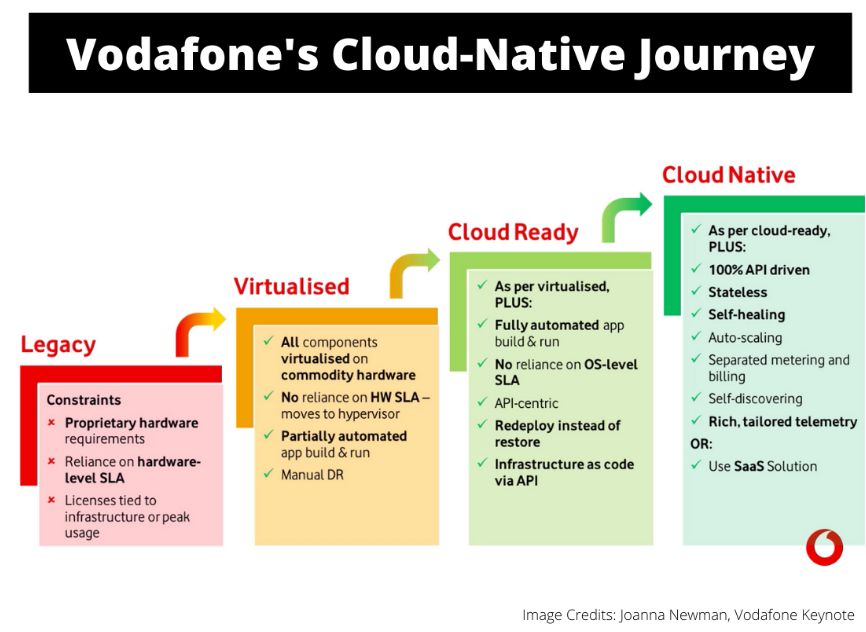
\includegraphics[width=\linewidth]{Images/vodafone}
		\end{figure}
		\end{column}
		\begin{column}[T]{4cm} % alternative top-align that's better for graphics
\begin{itemize}
	\item Nuevo SDLC
\item Automatización
\item Operación
\end{itemize}
		\end{column}
	\end{columns}
\end{frame}


\begin{frame}
	
	\begin{columns}
		
		% Primera columna
		\begin{column}{0.5\textwidth}
			\begin{itemize}
				\item \faCode ~ Código Base - Workflow definido, despliegue multientorno
				\item \faBox ~ Dependencias - Gestión y aislamiento
				\item \faCogs ~ Configuración - Externalización de parametros
				\item \faDatabase ~ Servicios backend  - Recursos acoplables
				\item \faCube ~ Construir, Liberar, Ejecutar - CI/CD 
				\item \faPlayCircle ~ Procesos - Aplicaciones sin estado
			\end{itemize}
		\end{column}
		
				
		% Segunda columna
		\begin{column}{0.5\textwidth}
			\begin{itemize}
				\item \faShip ~ Asignación de Puertos - No depender de servidor, autoexponerse a través de la red
				\item \faTasks ~ Concurrencia - Escalar horizontalmente
				\item \faCloud ~ Descartabilidad - Iniciar y caer de forma rápida y segura
				\item \faEquals ~ Dev/Prod Paridad - Entornos lo más similares posibles
				\item \faTerminal ~ Logs - Flujos de eventos hacia sistemas de agregación
				\item \faMedal ~ Procesos Admin - Operaciones administrativas idempotentes
			\end{itemize}
		\end{column}

	\end{columns}
\end{frame}

\begin{frame}
	
	\begin{columns}
		
		% Primera columna
		\begin{column}{0.5\textwidth}
			\begin{itemize}
				\item \faCode ~ Código Base - Gitflow, \textbf{Trunk Based}
				\item \faBox ~ Dependencias - \textbf{Maven}, NPM
				\item \faCogs ~ Configuración - AWS SSM, HashiCorp Vault, Kubernetes Secrets
				\item \faDatabase ~ Servicios backend  - S3, RDS
				\item \faCube ~ Construir, Liberar, Ejecutar - Jenkins, \textbf{Github Actions}
				\item \faPlayCircle ~ Procesos - \textbf{Quarkus}, Node.js
			\end{itemize}
		\end{column}
		
		
		% Segunda columna
		\begin{column}{0.5\textwidth}
			\begin{itemize}
				\item \faShip ~ Asignación de Puertos - \textbf{Vert.x}, Undertow, Kestrel
				\item \faTasks ~ Concurrencia - AWS Lambda, \textbf{Kubernetes}, ECS, Fargate
				\item \faCloud ~ Descartabilidad - \textbf{Docker}, Knative
				\item \faEquals ~ Dev/Prod Paridad - \textbf{Terraform}, Pulumi, Cloudformation, Docker
				\item \faTerminal ~ \textbf{Observabilidad} - \textbf{ServiceMonitors}, Opentelemetry, Cloudwatch, Grafana
				\item \faMedal ~ Procesos Admin - Flyway
			\end{itemize}
		\end{column}
		
	\end{columns}
\end{frame}

\begin{frame}
	
	\begin{columns}
		
		% Primera columna
		\begin{column}{0.2\textwidth}
\begin{figure}
	\centering
	
\includegraphics[width=\linewidth]{Images/tuxops}
	\label{fig:tuxops}
\end{figure}

		\end{column}
		
		
		% Segunda columna
		\begin{column}{0.8\textwidth}

{\LARGE ¿Y como controlo todo esto sin que me hackeen?}
		\end{column}
		
	\end{columns}
\end{frame}


	\section{DevSecOps}


\begin{frame}{DevOps}
	\begin{figure}
		\centering
		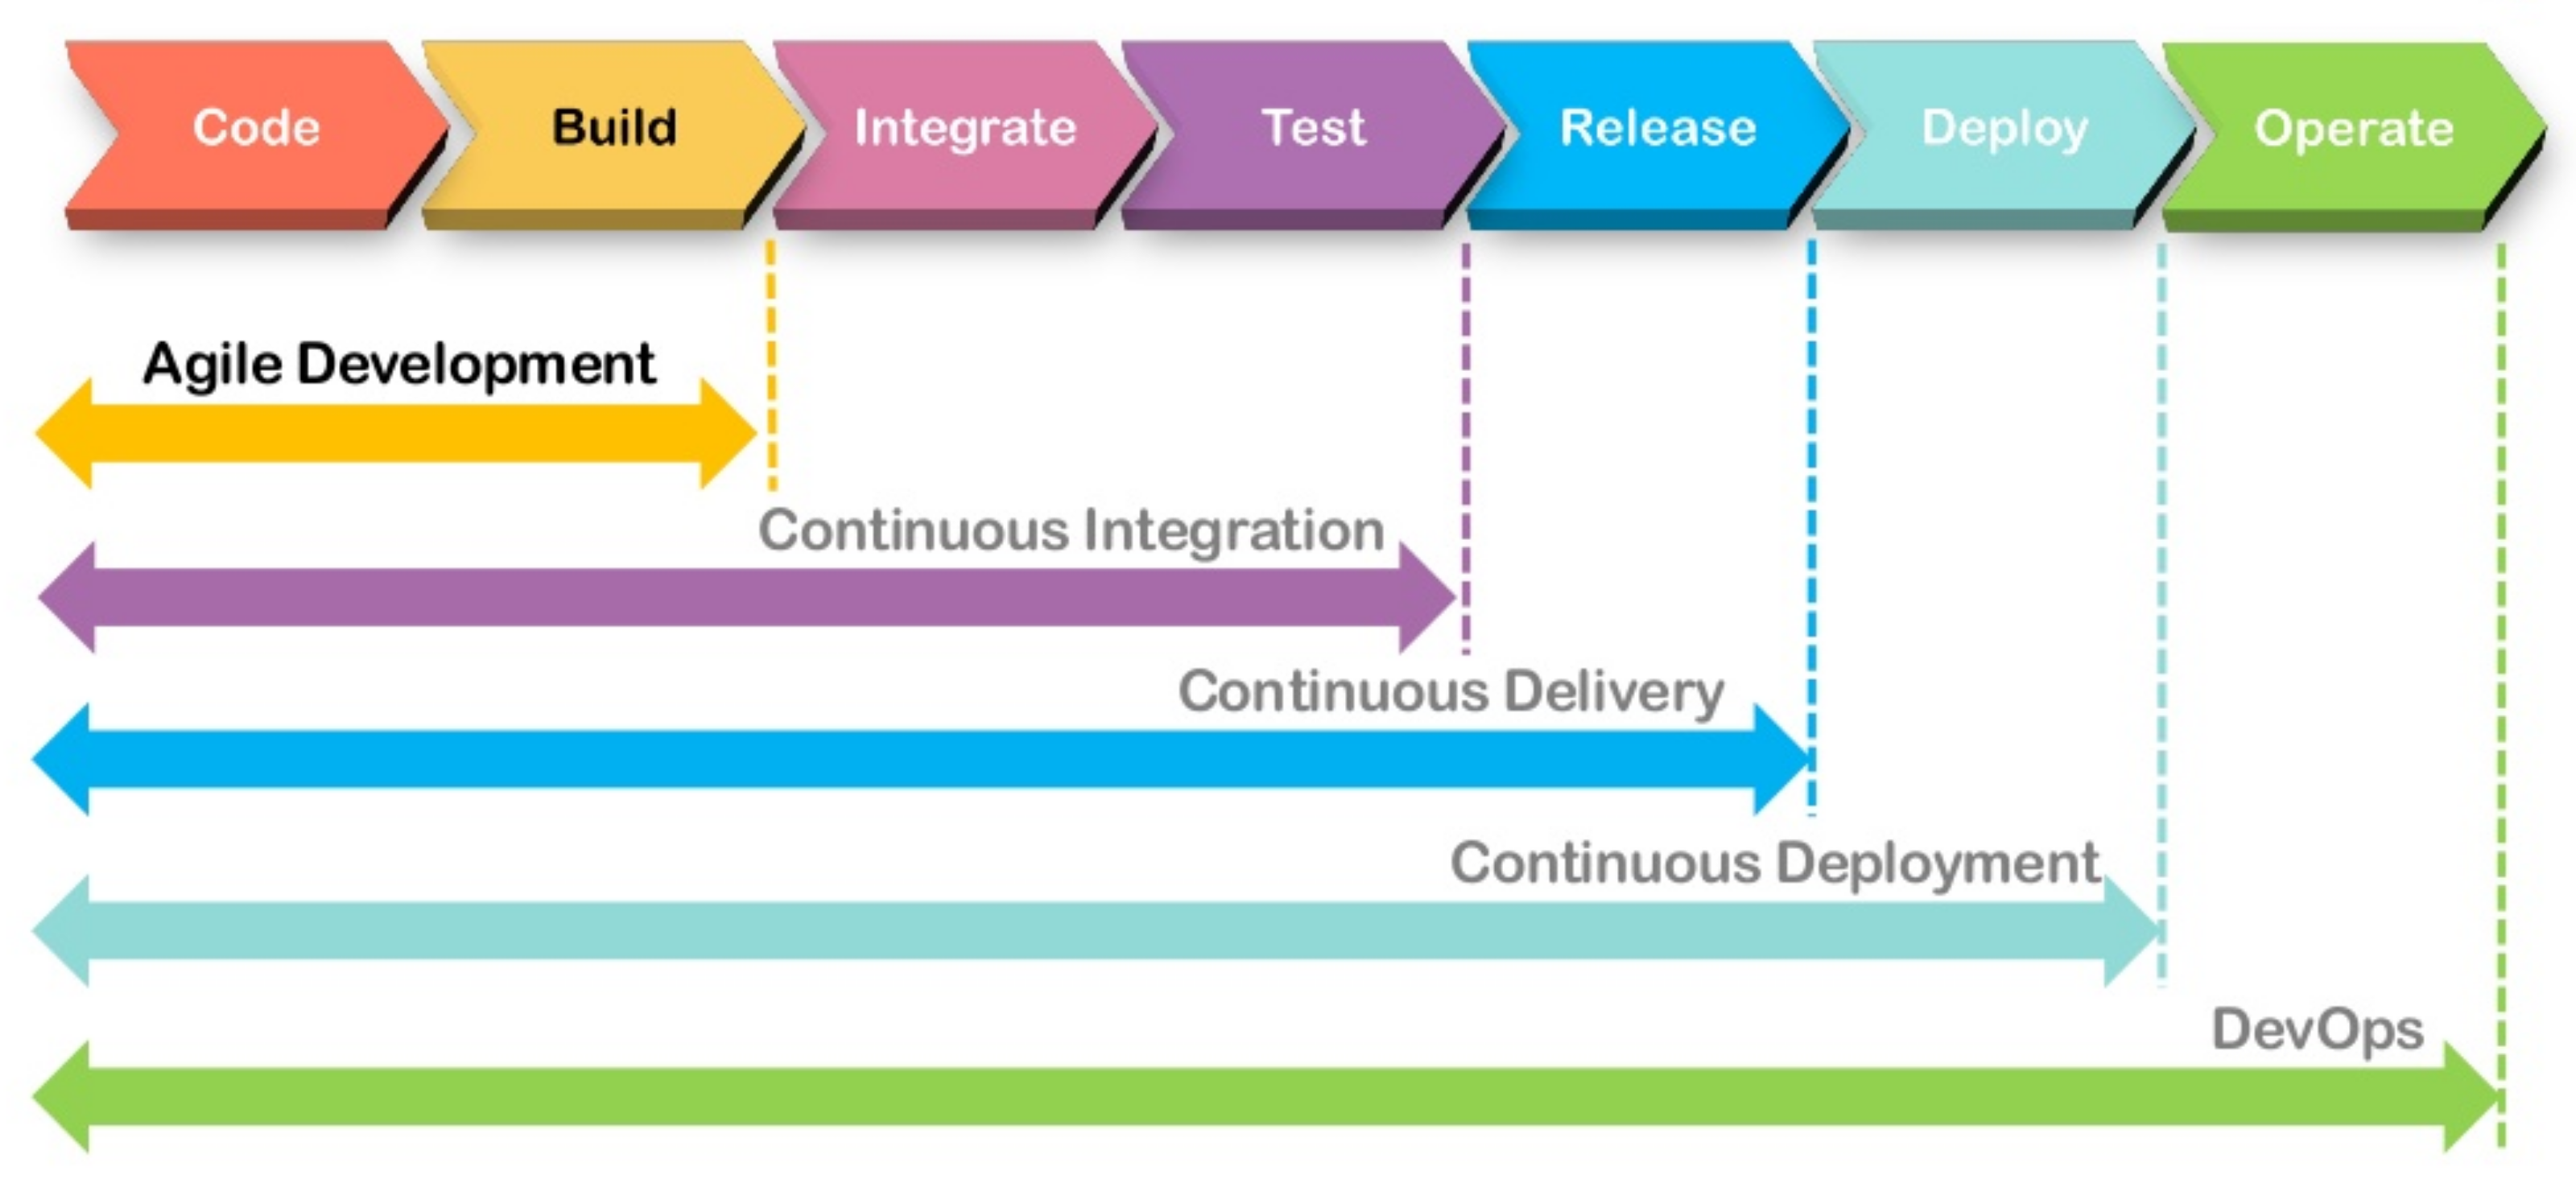
\includegraphics[width=\linewidth]{Images/etapa1}
		\label{fig:etapa1}
	\end{figure}
\end{frame}

\begin{frame}{Delivery vs Deployment}
	\begin{figure}
		\centering
		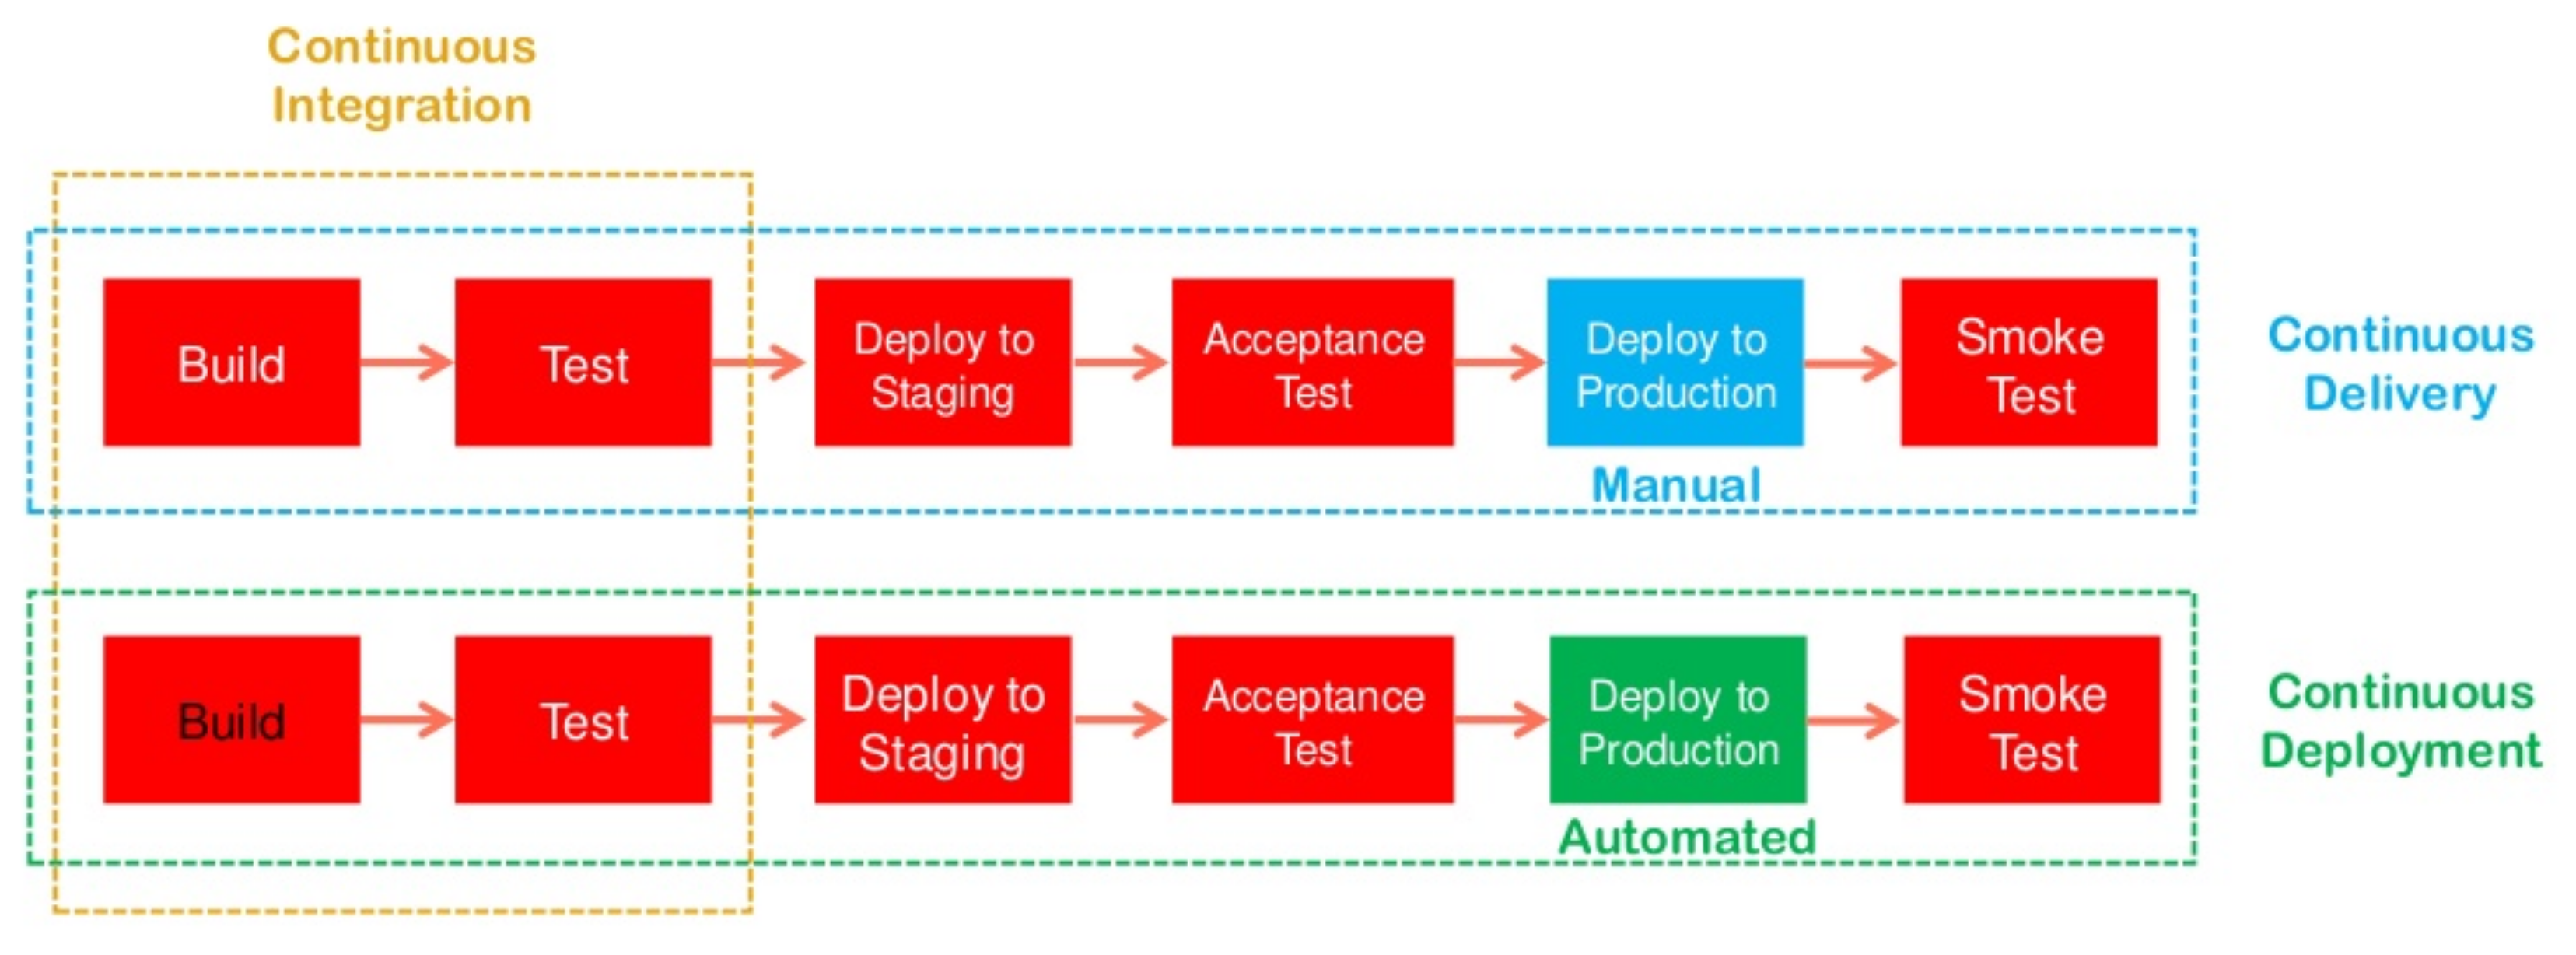
\includegraphics[width=\linewidth]{Images/etapa2}
		\label{fig:etapa2}
	\end{figure}
\end{frame}

\begin{frame}{DevSecOps}

	\begin{columns}
	
	% Primera columna
	\begin{column}{0.7\textwidth}
\begin{figure}
	\centering
	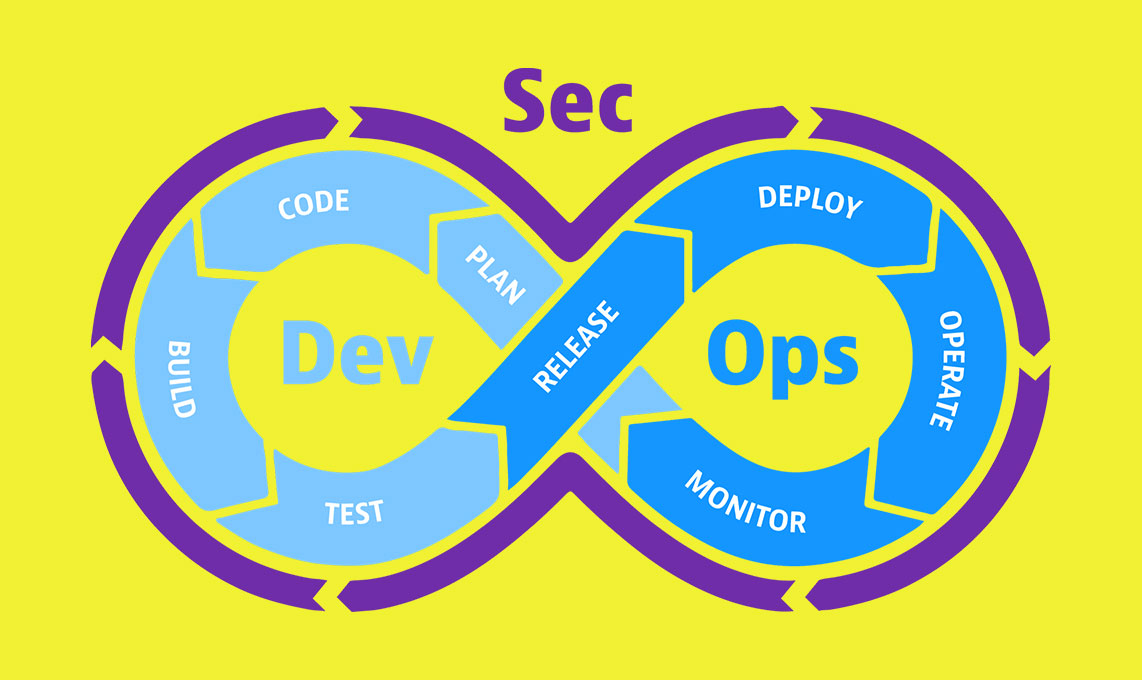
\includegraphics[width=\linewidth]{Images/etapa3}
	\label{fig:etapa3}
\end{figure}

	\end{column}
	
	
	% Segunda columna
	\begin{column}{0.3\textwidth}

\begin{itemize}
	\item Shift-Left
\item Automatización de pruebas
\item Security as code
\item Cumplimiento
\item Monitoreo y respuesta a incidentes
\end{itemize}		

	\end{column}
	
\end{columns}
\end{frame}

\begin{frame}{DevSecOps}
\begin{itemize}
	\item Shift-Left: Static Application Security Testing (Sonar, \textbf{Github Copilot}, \textbf{SpotBugs}), Software Composition Analysis (Snyk, Dependabot)
	\item Automatización de pruebas: DAST (OWASP ZAP) Container Security (AWS ECR Analysis, \textbf{Trivy} ), IaC
	\item Security as code: Cultura, capacitación constante (KnowBe4)
	\item Gestión de secretos y cumplimiento: AWS SSM, HashiCorp Vault, ISO 27001, SOC2, RBAC
	\item Monitoreo y detección en tiempo real: AWS Shield, AWS WAF, Falco, Crowdstrike
\end{itemize}		
\end{frame}

\begin{frame}{Ejemplo}
 \href{https://github.com/tuxtor/devsecops-walkthrough}{https://github.com/tuxtor/devsecops-walkthrough}

\end{frame}

\begin{frame}
\begin{figure}
	\centering
	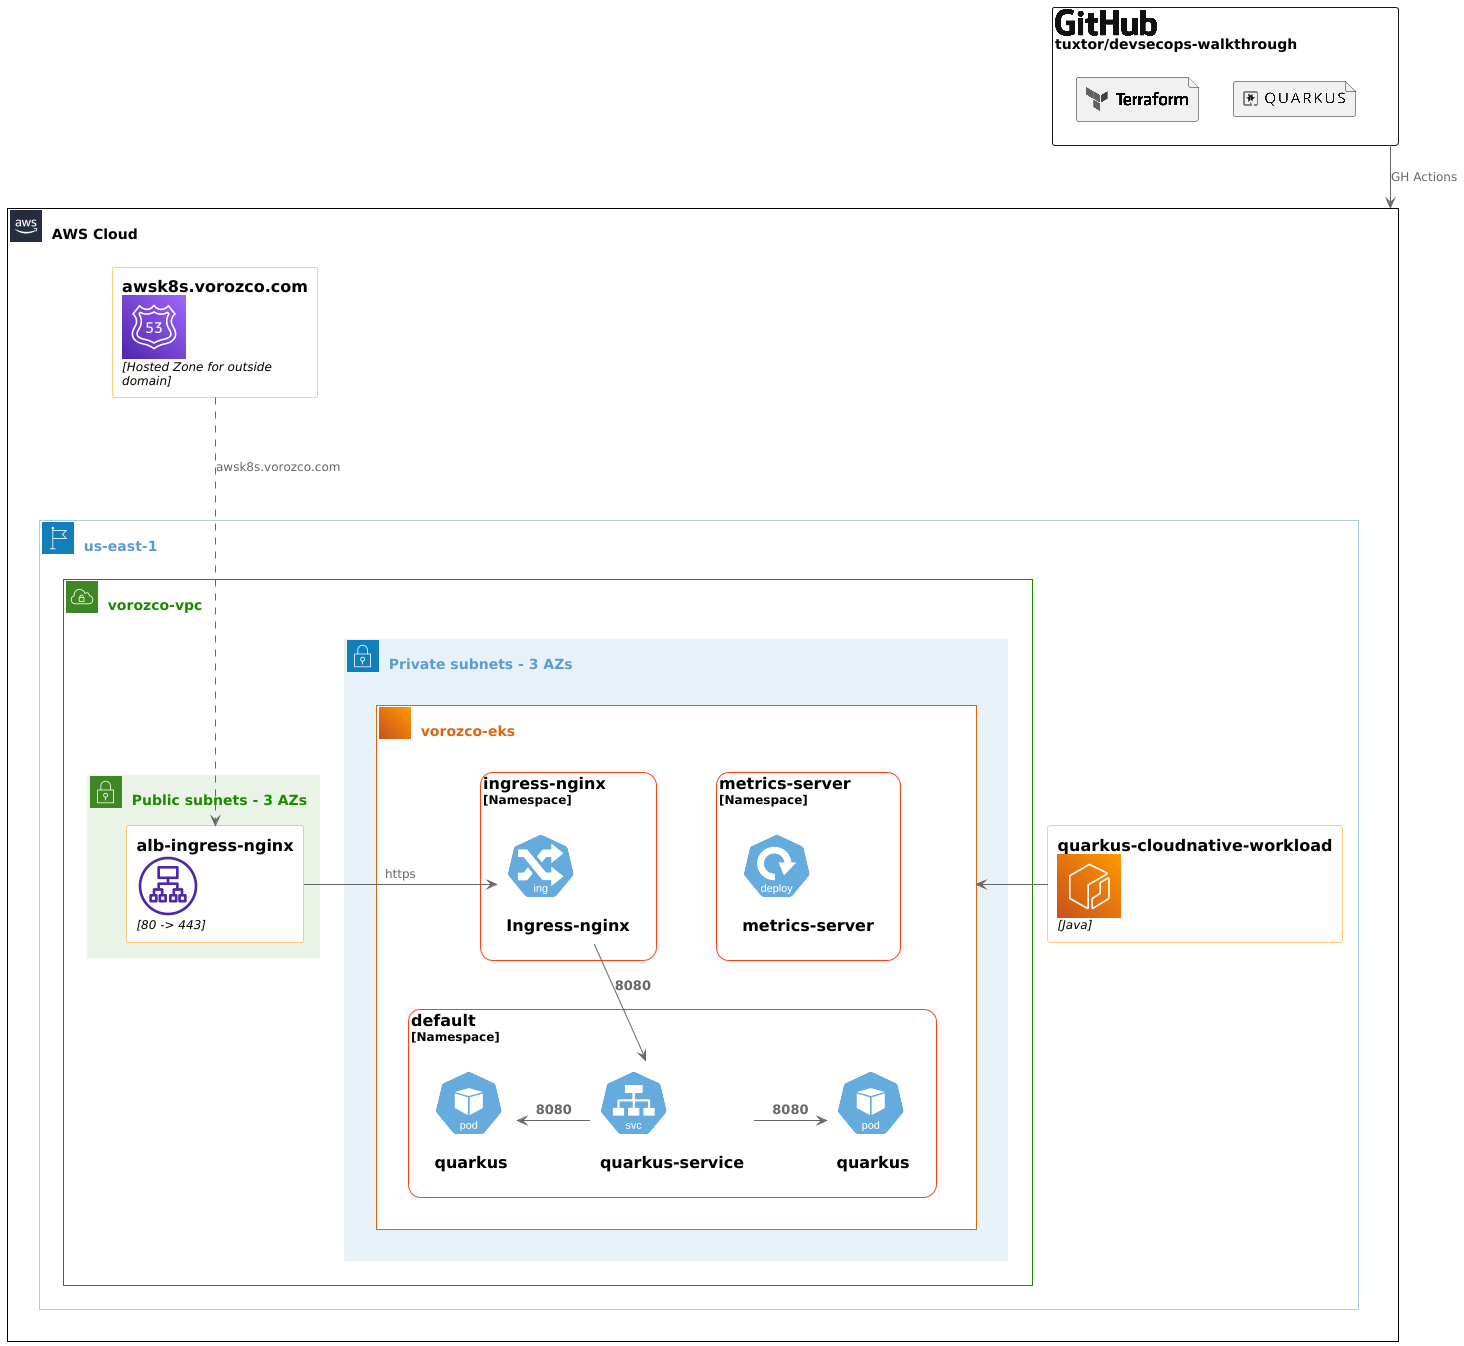
\includegraphics[width=0.7\linewidth]{Images/tuxops1}
	\label{fig:tuxops1}
\end{figure}

\end{frame}

\begin{frame}{¿Cómo hemos apoyado a otros clientes?}
	
	\begin{columns}[T]
		\begin{column}{0.5\textwidth}
			\begin{block}{Servicios de Consultoría}
				\begin{itemize}
					\item \faUserShield \hspace{0.2em} Implementación de infraestructura y pipelines CI/CD
					\item \faProjectDiagram \hspace{0.2em} Diseño e implementación de arquitecturas cloud native seguras
					\item \faCode \hspace{0.2em} Desarrollo E2E y de arquetipos
					\item \faGraduationCap \hspace{0.2em} Capacitación especializada para equipos
				\end{itemize}
			\end{block}
		\end{column}
		
		\begin{column}{0.5\textwidth}
			\begin{block}{Beneficios Clave}
				\begin{itemize}
					\item \faRocket \hspace{0.2em} Reducción de curva de aprendizaje
					\item \faGlobe \hspace{0.2em} Experiencia comprobada con proyectos alrededor del mundo
					\item \faMoneyBillWave \hspace{0.2em} Optimización de costos
					\item \faCertificate \hspace{0.2em} Conocimiento certificado
				\end{itemize}
			\end{block}
		\end{column}
	\end{columns}
	
	\centering
	\large{\textbf{Transformemos juntos tu ciclo de desarrollo con seguridad integrada}}
\end{frame}


\begin{frame}{Víctor Orozco}
	\begin{columns}[T] % contents are top vertically aligned
		
		\begin{column}[T]{4cm} % alternative top-align that's better for graphics
			\begin{figure}
				\centering
				
\includegraphics[width=0.8\linewidth]{Images/logos}
			\end{figure}
		\end{column}
		\begin{column}[T]{6cm} % each column can also be its own environment
			\begin{itemize}
				\item me@vorozco.com
				\item \href{https://twitter.com/tuxtor}{@tuxtor}
				\item \href{https://vorozco.com}{https://vorozco.com}
				\item \href{https://tuxtor.shekalug.org}{https://tuxtor.shekalug.org}
			\end{itemize}
			\begin{center}
				
\includegraphics[width=0.1\linewidth]{Images/cclogo}
				\\
				This work is licensed under Creative Commons Attribution-NonCommercial-ShareAlike 3.0 Guatemala (CC BY-NC-SA 3.0 GT).
			\end{center}
		\end{column}
	\end{columns}
\end{frame}



\end{document}

